Opgaven omhandler to-dimensionelle vektorer. En to-dimensionel vektor (herefter blot vektor) er et geometrisk objekt som består af en retning og en længde. Typisk repræsenteres vektorer som par af tal $\vec v  = (x, y)$, hvor længden og retningen findes ved,
\begin{align}
  \text{len}(\vec v) &= \sqrt{x^2+y^2}
  \\\text{ang}(\vec v) &=\text{atan2}(y, x)
\end{align}
Vektorens ender kaldes hhv.\ hale og spids, og når halen placeres i $(0, 0)$, så vil spidsen have koordinat $(x, y)$. Vektorer har en række standardoperatorer,
\begin{align}
  \vec v_1 &= (x_1, y_1)
  \\\vec v_2 &= (x_2, y_2)
  \\a \vec v_1 &= (a x_1, a y_1)
  \\\vec v_1 + \vec v_2 &= (x_1+x_2, y_1+y_2)
  \\\vec v_1 \cdot \vec v_2 &= x_1 x_2 +  y_1y_2
\end{align}
Addition kan tegnes som vist i \Cref{fig:vectorAddition}.
\begin{figure}
  \centering
  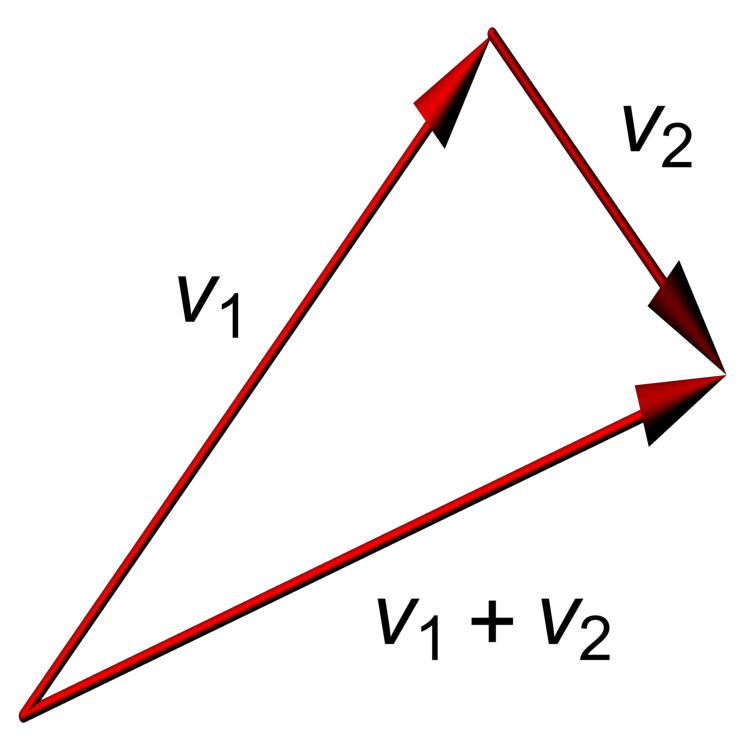
\includegraphics[width=0.33\textwidth]{vectorAddition}
  \caption{Illustration of vector addition in two dimensions.}
  \label{fig:vectorAddition}
\end{figure}
